This chapter will show use cases showing how the simulator can be used.

\section{Use case 1}
	\subsection*{2 Versus 2}
	This first use case will show a battle between 2 teams each having the same regiments.
	The first team is a group of Pirates and the other team is a group of Ninjas. The grid is a $4 \times 4$ map. \\
	Team Pirates are shown here. The regiments are also present in the Ninja team file, but with names starting with Ninja.
\begin{lstlisting}
Regiment PirateArcher
{
	Size = 10;
	Type = Ranged;
	Range = 2;
	Damage = 4;
	Health = 4;
	Movement = 1;
	AttackSpeed = 1;
	RegimentPosition = Position(4,5);
	Behaviour ArcherBehaviour
	{
		Regiment enemy = SearchForEnemies();
		if (enemy.Distance <= Range)
		{
			Attack(enemy);
			if(enemy.Distance < 2)
			{
				MoveAway(enemy);
			}
		}
		else
		{
			MoveTowards(enemy);
		}
	}
}
Regiment PirateWarrior
{
	Size = 10;
	Type = Melee;
	Damage = 8;
	Health = 4;
	Movement = 1;
	AttackSpeed = 1;
	RegimentPosition = Position(2,5);
	Behaviour WarriorBehaviour
	{
		Regiment enemy = SearchForEnemies();
		if (enemy.Distance <= Range)
		{
			Attack(enemy);
		}
		else
		{
			MoveTowards(enemy);
			Attack(enemy);
		}
	}
}
\end{lstlisting}

	\subsection*{Screenshots from use case 1}
		\begin{figure}[H]
			\center
			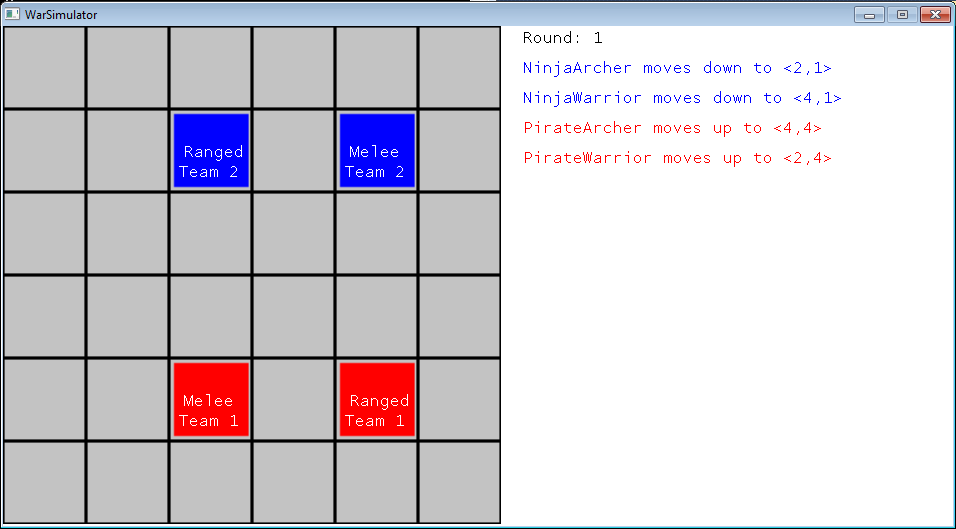
\includegraphics[scale=0.6]{rapport/7/figures/case1-1.png}
			\caption{The battle begins}
		\end{figure}
		\begin{figure}[H]
		\center
			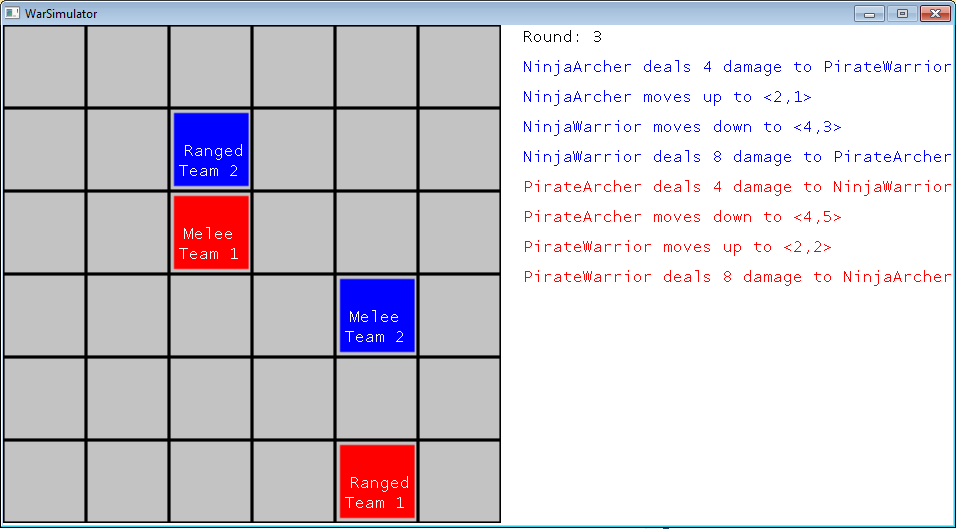
\includegraphics[scale=0.6]{rapport/7/figures/case1-2.png}
			\caption{The Warriors chase the archers}
		\end{figure}
		\begin{figure}[H]
		\center
			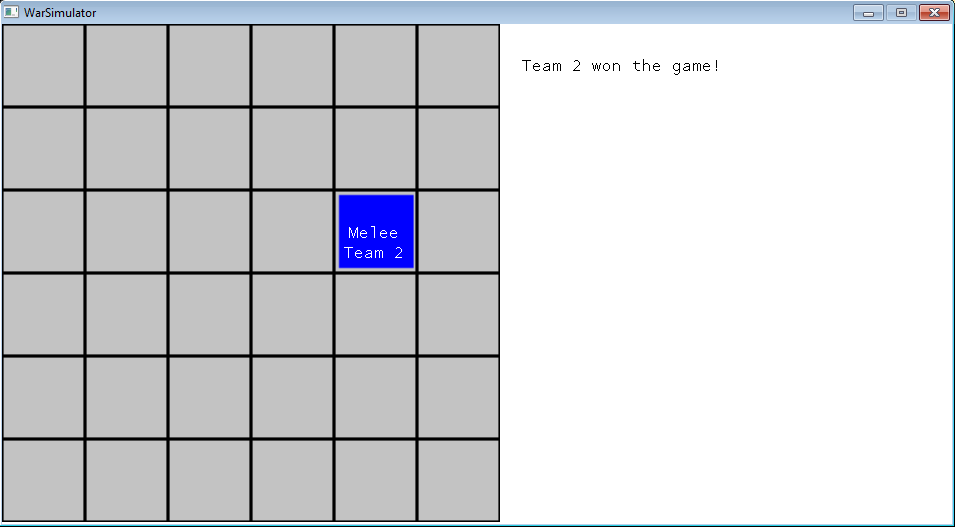
\includegraphics[scale=0.6]{rapport/7/figures/case1-3.png}
			\caption{Team 2 won!}
		\end{figure}
		
\section{Use case 2}
	\subsection*{Big battle}
	This use case will show a big battle between 4 teams. This scenario also showcases how the grid will scale when the 
	grid size is increased. In this battle the grid size is $10 \times 10$
	
	\subsection*{Screenshots from use case 2}
		\begin{figure}[H]
			\center
			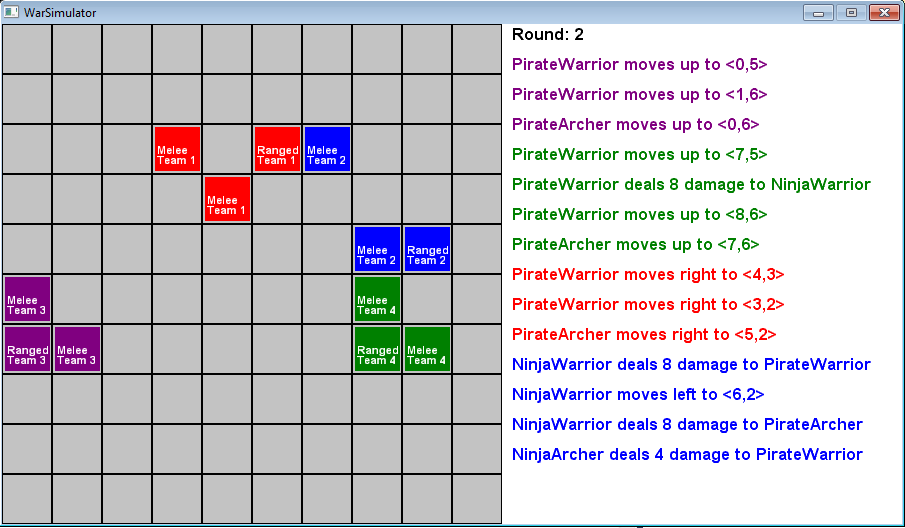
\includegraphics[scale=0.6]{rapport/7/figures/case2-1.png}
			\caption{The battle begins}
		\end{figure}
		\begin{figure}[H]
		\center
			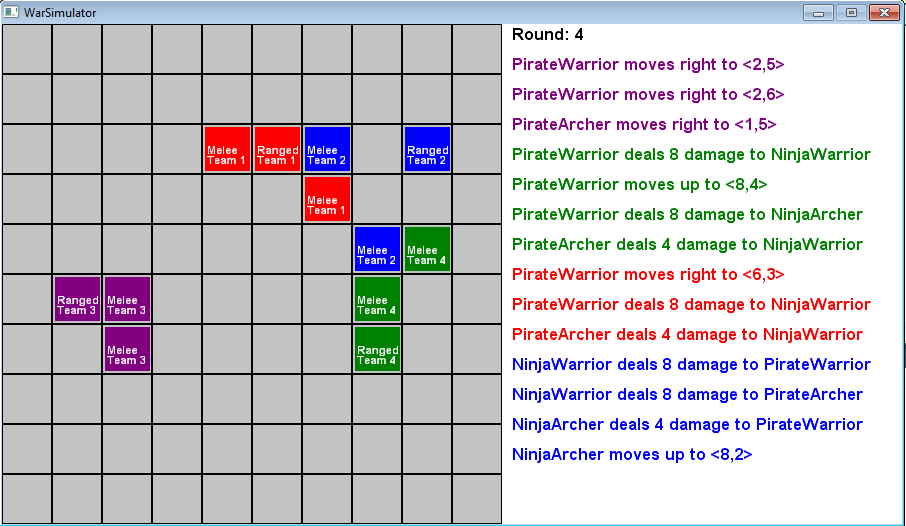
\includegraphics[scale=0.6]{rapport/7/figures/case2-2.png}
			\caption{Team 3 is being passive}
		\end{figure}
		\begin{figure}[H]
		\center
			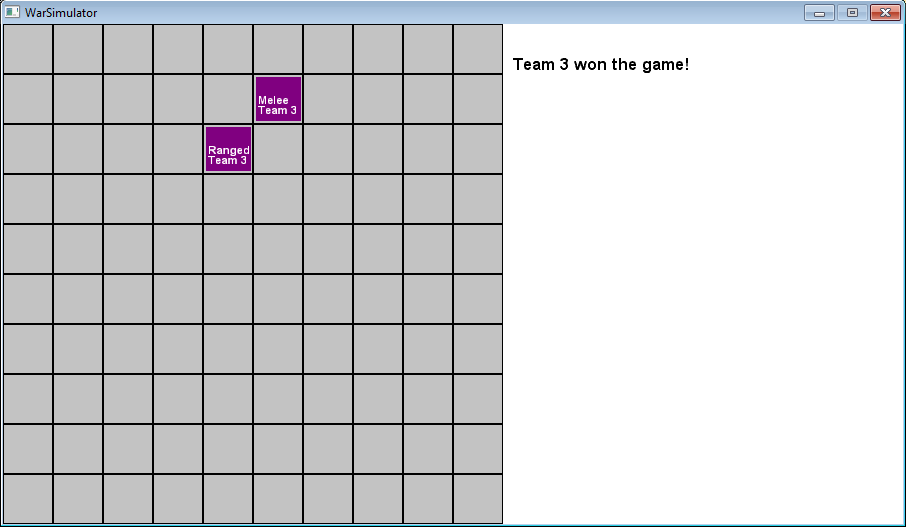
\includegraphics[scale=0.6]{rapport/7/figures/case2-3.png}
			\caption{Team 3 won!}
		\end{figure}